% !TeX spellcheck = da_DK
\subsection{Forstærker i tilpasningsblok}
\subsubsection{Teori og design}
I afsnit \ref{Subsec:Forstaerker}, side \pageref{Subsec:Forstaerker} er teorien samt designet af en forstærker forklaret. Da blokken tilpasning skal tilpasse det filtrerede signal til komparatoren, afgrænses måleintervallet til $\pm25^{\circ}$. Et range på $\pm90^{\circ}$ er unødvendigt ift. at vurdere hvorvidt patienten er faldet. Derfor ønskes det, at $V_{out}$ fra denne blok er $\pm3$V, når accelerometret måler $\pm25^{\circ}$. Der skal dermed ske en forstærkning med en faktor $3.6$, hvilket svarer til $11.1261$dB, som beskrevet i afsnit \ref{Tilpasningsblok} på side \pageref{Tilpasningsblok}. \\
For at udregne modstandene er R$2$ blevet valgt til $10$K$\Omega$. Ud fra dette er R$1$ blevet bestemt ved følgende udregning:
\begin{equation}
3.6 = 1 + (\frac{R1}{10\text{K}\Omega}) \\
R1 = 26\text{K}\Omega
\end{equation}

\noindent Forstærkerens opbygning kan ses på \figref{fig:Forstaerker_faktor3}.
\begin{figure}[H]
	\centering
	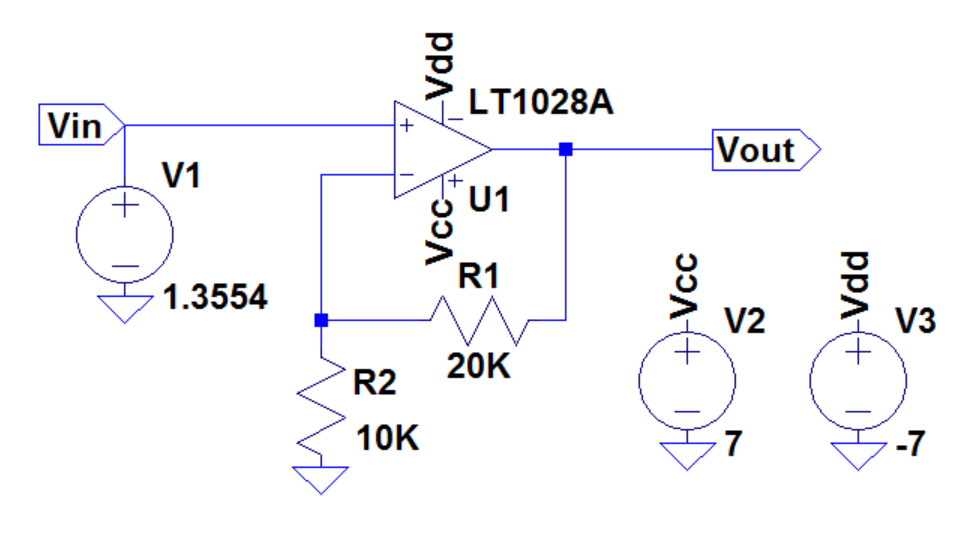
\includegraphics[scale=0.3]{figures/cProblemloesning/Forstaerker_faktor3.PNG}
	\caption{På figuren ses opbygningen af den ikke-inverterende forstærker, der forstærker med en faktor $3.6$.}
	\label{fig:Forstaerker_faktor3}
\end{figure}

\subsubsection{Simulering}
Forstærkeren testes i fire simuleringer for at undersøge, om den opfylder de opstillede krav. Det forstærkede signal($V_{out}$), skal være $3.6$ gange større end blokkens inputsignal($V_{in}$). Resultaterne af fire simuleringer ses i \tableref{tab:forstarker3_simT}. Der er benyttet de teoretiske værdier, som er udregnet fra start.
\begin{table}[H]
	\centering
	\begin{tabular}{|l|l|l|l|l|l|}
		\hline
		\multicolumn{1}{|c|}{\textit{Inputsignalet}} & \multicolumn{1}{c|}{\textit{Forstærkning}} & \textit{\begin{tabular}[c]{@{}l@{}}Forventet\\outputsignal\end{tabular}} & \multicolumn{1}{c|}{\textit{Outputsignalet}} & \textit{Forstærkning}  & \multicolumn{1}{c|}{\textit{Afvigelse}} \\ \hline
		$3.0148$V     & $3.6$   & \begin{tabular}[c]{@{}l@{}}Forventer mætning\\ $10.8533$V\end{tabular} & $3.9765$V  & $\times$ & $\times$     \\ \hline
		$0.8418V$V    & $3.6$   & $3.0305$V                                                              & $3.0304$V  & $3.6$ & $0\%$     \\ \hline
%		$0$V          & 3   & $0$V                                                                   & $33.6527\mu $V        & $\approx 0\%$     \\ \hline
	   -$0.8190$V     & $3.6$   & -$2.9484$V                                                             & -$2.9482$V  & $3.6$ & $0\%$     \\ \hline
	   -$2.9420$V     & $3.6$   & \begin{tabular}[c]{@{}l@{}}Forventer mætning\\ -$10.5912$V\end{tabular}& -$3.97703$V  & $\times$ & $\times$     \\ \hline
	\end{tabular}
		\caption{I tabellen ses resultaterne af de fire simuleringer.}
		\label{tab:forstarker3_simT}
\end{table}
\indent Der ses i \tableref{tab:forstarker3_simT}, at der er en lav afvigelse er i forstærkningen, men dette lægger inde for referencerne. Kredsløbet fungerer rent teoretisk med ideelle komponenter, som bliver brugt i LTspice. På \figref{fig:faktor3_simulering} ses simuleringen af et inputsignal på $0.8325$V, som ideelt vil komme fra filtreringsblokken, hvis accelerometret hælder i $25^{\circ}$.

\begin{figure}[H]
	\centering
	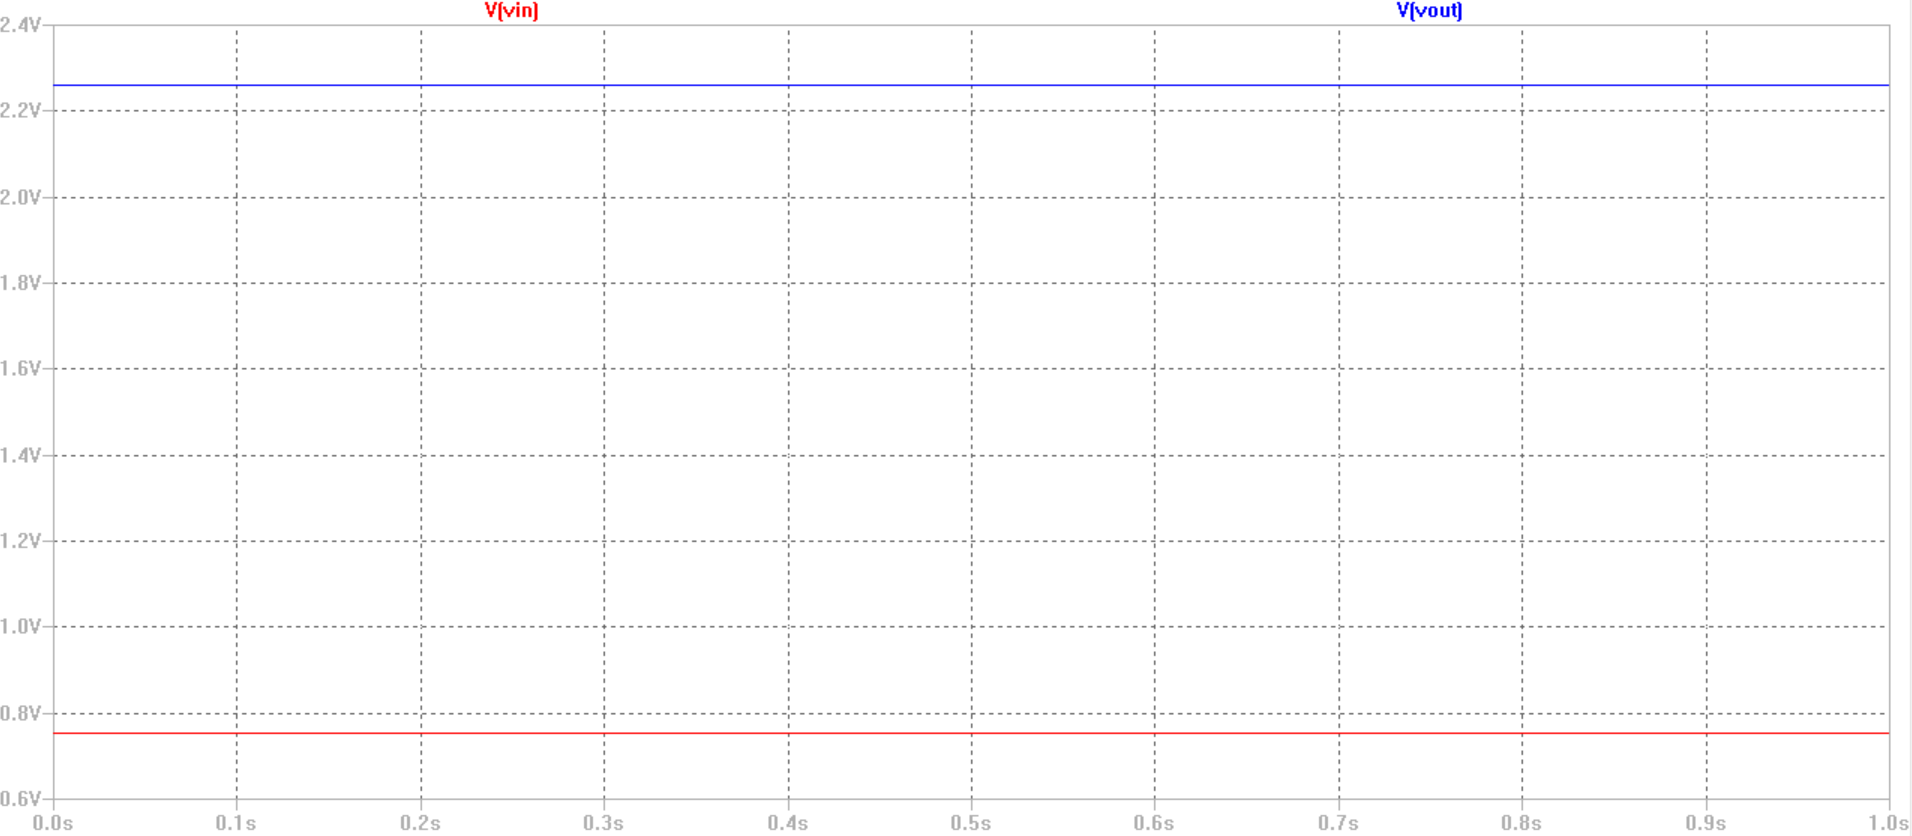
\includegraphics[scale=0.3]{figures/cProblemloesning/Forstaerker_faktor3_simulering.PNG}
	\caption{På figuren ses simuleringen for et inputsignal på $0.8418$V, som giver $3.0304$V i output. Der er således sket en forstærkning med en faktor $3.6$.}
	\label{fig:faktor3_simulering}
\end{figure}
\noindent Der ses på afvigelserne, at der arbejdes med ideelle komponenter. Det er herved bevist, at kredsløbet fungerer teoretisk og kan derfor implementeres.

\subsubsection{Implementering og test}
På \figref{fig:Forstaerker_faktor3} kan der ses, at der skal benyttes to modstande på $10$K$\Omega$ og $26$K$\Omega$ til opbygningen af forstærkeren. Reelt findes der dog ikke en $26$K$\Omega$, hvorfor der istedet benyttes $27$K$\Omega$- og $680$K$\Omega$ modstande i parallel forbindelse, hvilket teoretisk vil give en $0.12$\% afvigelse fra en ideelt $26$K$\Omega$ modstander. Disse tre modstande blev målt inden implementering, hvilket fremgår i \tableref{Tab:modstand_faktor18}.
\begin{table}[H]
	\centering
	\begin{tabular}{|l|l|l|}
		\hline
		\textit{Teoretisk}  & \textit{Ved måling} & \textit{\% afvigelse} \\ \hline
		$10$K$\Omega$       & $9.98$K$\Omega$     & $0.2$\%               \\ \hline
		$680$K$\Omega$      & $684.53$K$\Omega$   & $0.67$\%               \\ \hline
		$27$K$\Omega$       & $26.99$K$\Omega$    & $0.4$\%               \\ \hline
	\end{tabular}
	\caption{I tabellen ses det, at de tre modstande har en lille afvigelse fra deres teoretiske værdi, hvilket er forventet af reelle komponenter. Det er en acceptabel afvigelse, og modstandene kan derfor anvendes i implementeringen.}
	\label{Tab:modstand_faktor18}
\end{table}

\noindent Herefter implementeres kredsløbet. Til afbildning af signalet blev benyttet et multimeter. De aflæste resultater for spændingen efter forstærkningen er angivet under "Output" i \tableref{Tab:faktor3_test}.\

\begin{table}[H]
	\centering
	\begin{tabular}{|l|l|l|l|l|l|}
		\hline
 \textit{\begin{tabular}[c]{@{}l@{}}Ønsket\\input\end{tabular}} & \textit{Input} & \textit{Forventet output} & \textit{Output}  &  \textit{Forstærkning}  & \% afvigelse \\ \hline
   $3.0148$V &  $3.0146$V           & \begin{tabular}[c]{@{}l@{}}mætning\\ $10.8526$V\end{tabular}  & $4.8403$V   &    $\times$     & $\times$  \\ \hline
   $0.8418$V &  $0.8417$V           & $3.0301$V                                                     & $3.0286$V   &    $3.6$        & $0\%$     \\ \hline
  -$0.8190$V & -$0.8192$V           & -$2.9491$V                                                    & -$2.9584$V  &    $3.61$       & $0.28\%$     \\ \hline
  -$2.9420$V &-$2.9439$V            & \begin{tabular}[c]{@{}l@{}}mætning\\ -$10.5980$V\end{tabular} & -$4.1651$V  &    $\times$     & $\times$    \\ \hline
	\end{tabular}
	\caption{I tabellen ses resultaterne fra testen med forstærkeren med en faktor $3.6$.}
	\label{Tab:faktor3_test}
\end{table}
Det ses i \tableref{Tab:faktor3_test}, at forstærkeren overholder kravene fra afsnit \ref{OpsamlingsAfs} på side \pageref{OpsamlingsAfs} samt ligger inde for tolerancerne. Derfor anses disse afvigelser som acceptable.